\documentclass[11pt,a4paper,titlepage]{report} 
\usepackage[utf8]{inputenc} 
\usepackage[french]{babel} 
\usepackage[T1]{fontenc} 
\usepackage{amsmath} 
\usepackage{amsfonts} 
\usepackage{amssymb} 
\usepackage{graphicx} 
\usepackage[final]{pdfpages} 
\usepackage[toc,page]{appendix} 
\usepackage[top=2.5cm,bottom=2.5cm,right=2.5cm,left=2.5cm]{geometry} 
\usepackage{minted}
\author{GLANGINE Geoffrey} 
\title{Simulateur de vente de billet de cinéma} 
\graphicspath{{Images/}} 
\usepackage{fancyhdr} 
\pagestyle{fancy} 
\usepackage{lastpage} 
\renewcommand
\headrulewidth{1pt} 
\fancyhead[L]{Systèmes d'exploitation} 
\fancyhead[C]{GLANGINE Geoffrey} 
\fancyhead[R]{LO41 UTBM} 
\renewcommand
\footrulewidth{1pt} 
\fancyfoot[C]{\textbf{Page \thepage}} 
\fancyfoot[L]{Automne 2015}

\newcommand{\HRule}{\rule{\linewidth}{0.5mm}}

\begin{document}

\begin{titlepage}
\begin{center}

% Upper part of the page. The '~' is needed because \\
% only works if a paragraph has started.
%\includegraphics[width=0.15\textwidth]{./logo}~\\[1cm]

\textsc{\LARGE Université de technologie Belfort-Montbéliard}\\[1.5cm]

\textsc{\Large Simulateur de vente de billet de cinéma}\\[0.5cm]

% Title
\HRule \\[0.4cm]
{ \huge \bfseries LO41 Système d'Exploitation : Principes et Communication\\[0.4cm] }

\HRule \\[1.5cm]

% Author and supervisor
\begin{minipage}{0.4\textwidth}
\begin{flushleft} \large
\emph{Auteur:}\\
\textsc{GLANGINE} Geoffrey\\
\end{flushleft}
\end{minipage}
\begin{minipage}{0.4\textwidth}
\begin{flushright} \large
\emph{Professeur:} \\
\textsc{DESCAMPS} Philippe
\end{flushright}
\end{minipage}
\vfill
\begin{figure}[h]
 
\includegraphics[width=16cm]{cinema.jpg}
\end{figure}
\vfill
% Bottom of the page
{\large \today}

\end{center}
\end{titlepage}
\pagebreak
\tableofcontents
\pagebreak

\chapter{Introduction}
Dans le cadre de l'UV LO41 dispensée à l'UTBM, un projet de gestion de vente de billet dans un Cinéma a été donné.
Après une analyse du sujet, j'aborderai les objectifs que je me suis fixé, ceux que j'ai réussi à implémenter ainsi
que ceux que je n'ai pas réussi à implémenter.
\chapter{Analyse du sujet}
\section{Sujet}
L'analyse du sujet m'a conduit à penser qu'il fallait que je fasse des thread Clients qui arrivent en plusieurs ou une seule grosse vague. Ainsi que des thread pour les caissières. Dans mon analyse de code, je pensais 
faire choisir le film dans le thread de la caissière, mais l'implémentation m'a conduit à faire choisir le film dans le thread du client.

Ainsi les caissières ne disposent d'aucune information sur les clients.  

\section{Objectifs}
\subsection{Les objectifs fixés :}
\begin{itemize}
 \item Je souhaitais pouvoir gérer un très grand nombre de clients à la fois (car on ne sait pas le nombre de clients qui peuvent arriver en même temps dans un Cinéma)
 \item Je souhaitais aussi que le nombre de salles dans mon Cinéma ne soit pas limité par une quelconque valeur. (En effet dans un cinéma il y a souvent plusieurs salles fermées qui peuvent être ouverte dans le cas ou il y a beaucoup de monde.)
 \item Je voulais pouvoir paramétrer toute les variables sans avoir à recompiler à chaque fois
 \item Je voulais aussi que les personnes attendent devant la salle que les précédentes personnes sortent, entrent dans les salles regardent le film en fonction de la durée du film et qu'ils sortent ensuite du cinéma. 
 \end{itemize}

 \subsection{Les moyens pour parvenir à mes objectifs}
\begin{itemize}
 \item Pour le grand nombre de client, en C c'est très facile de générer beaucoup de thread. Il suffit juste de les ordonnancer correctement.
 \item Le nombre de salle Ouvertes dans mon cinéma n'est pas fixe. En effet mes salles sont répertoriées dans une liste chaînée.
 \item Pour modifier les valeurs de base de mon projet, j'ai crée un fichier de configuration au format XML en utilisant la librairie libxml2.
 \item Synchronisation de mes thread à l'aide de moniteurs 
 \begin{itemize}
  \item Un Thread par caisse
  \item Un Thread par Client
  \item Un Thread pour gérer le début de la séance
 \end{itemize}

 \item Utilisation des signaux pour bloquer l'interruption et nettoyer la mémoire / les threads à la sortie du programme.
\end{itemize}

\subsection{Objectifs atteints}
J'ai atteins tous les objectifs expliqués dans la partie précédente sauf le fait que les personnes entre dans les salles regardent un film d'une certaine durée et sortent du cinema à la fin. En effet j'ai une seconde version du projet qui a cette
cette fonctionnalité d'implémentée mais elle est buggée. Dans certains cas plus ou moins rares mes threads restent bloqués dans une situation d'inter-blocage et le programme ne se termine jamais.
Du fait de la rareté du bug et de la manière difficile de le déboguer je n'ai pas pu le résoudre. J'ai donc prévu de rendre un projet propre et fonctionnel plutôt qu'une version "Améliorée" qui ne fonctionne pas de manière sure.
\subsection{Nettoyage de la mémoire}
Au niveau du nettoyage de la mémoire je libère tout l'espace mémoire à la fin de mon programme et l'interrompt tous les threads qui tournent encore si l'on fait un ctrl+c.

\subsection{Difficultés rencontrées}

\begin{itemize}
 \item Problème d'inter-blocage, Comme parlé plus haut, je me suis retrouvé confronté à un problème d'inter-blocage, ce qui m'a conduit à devoir réduire la quantité de fonctionnalités que je voulais implémenter. de plus ce genre de problème est très dur à résoudre car l'utilisation du débogueur est impossible.
\end{itemize}

\chapter{Conception}
\section{La structure du programme}
\subsection{Réseau de pétri :}

Durant ma phase d'analyse, j'ai représenté un réseau de pétri pour avoir un support sur lequel m'appuyer pour voir le fonctionnement de la synchronisation de mes threads. :
Le schéma ci dessous représente un cas avec une seule caisse, pour des raisons de simplifications du schéma. 

\begin{figure}[h]
 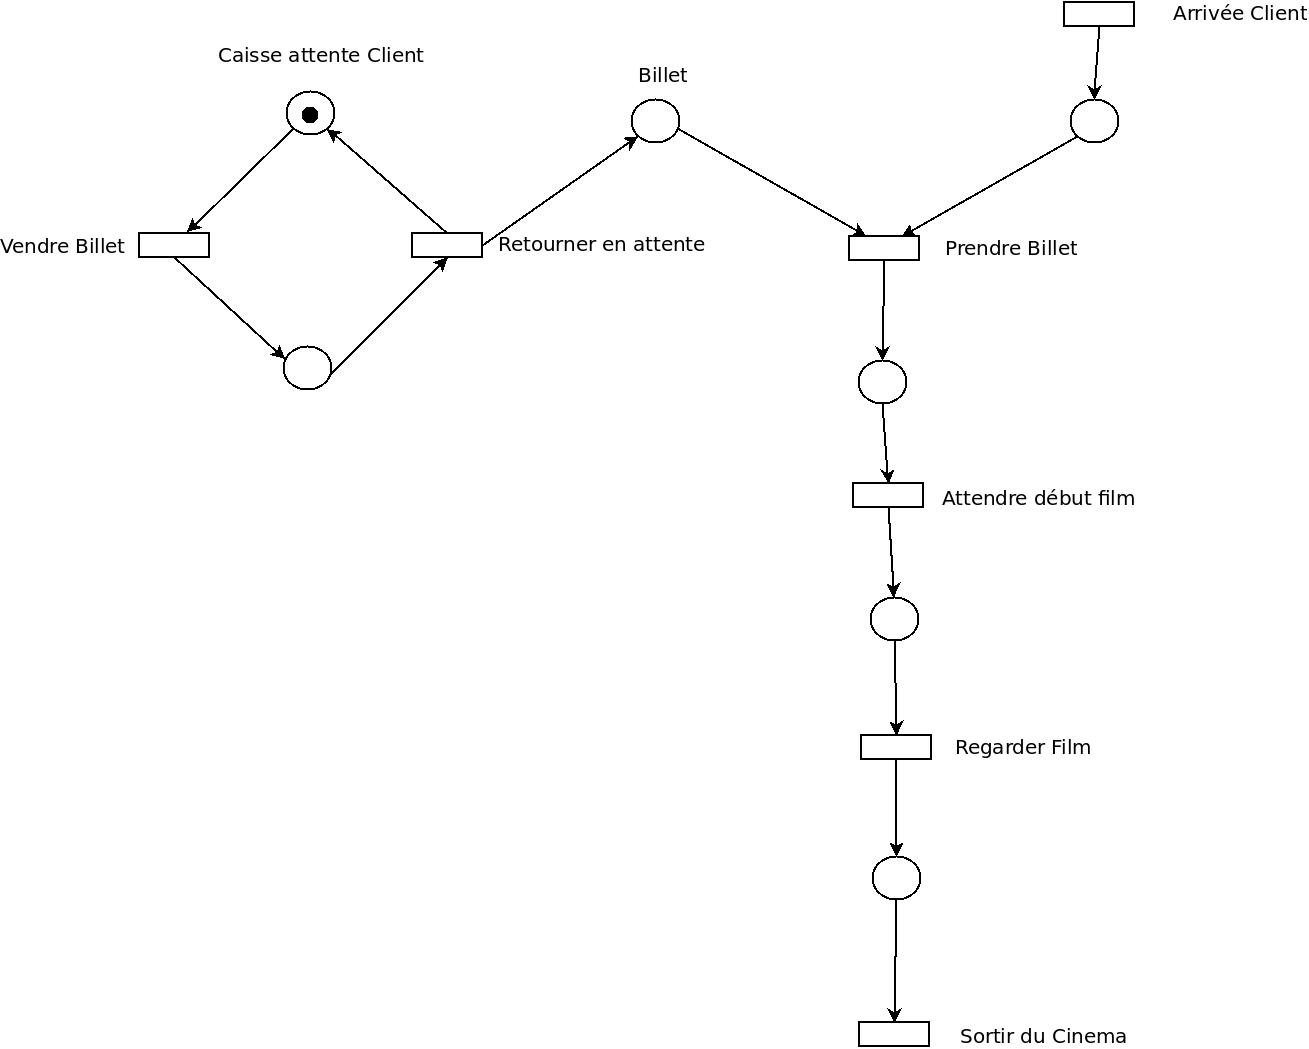
\includegraphics[width=15cm]{petri.jpeg}
\end{figure}
\pagebreak

\subsection{Les structures et variables globales}

les différents "objets" sont décris avec des structures En voici une description : 

\begin{minted}{C}
 
 typedef struct FilmStruct{
    
    char *titre;
    char *genre;
    int duree;
    int horaire;
    int pegi;
    int id;
    int NbPlaceRefuse;
    
}FilmStruct;
  
\end{minted}

La structure FilmStruc permet de représenter un Film par un nom, un genre, une durée, un horaire, un age requis (norme PEGI), un identifiant, et un Nombre de place refusées pour compter les personnes qui n'on pas pu voir ce film. Au bout d'un certain nombre, si il reste des salles libres, on ouvre une nouvelle salle avec ce film.

\begin{minted}{C}

  typedef struct SalleStruct{
    int CAPACITE;
    int NBPersonnes;
    FilmStruct * film;
    int numero;
    
}SalleStruct;

\end{minted}

Ma seconde structure est la structure SalleStruct qui permet de représenter une salle par une capacité, un nombre de personnes, un film,et un numéro.

\subsubsection{Les variables Globales : }

\begin{minted}{C}
pthread_t* tid; //tableau des threads client et caisses
pthread_t* threadManagement; //tableau des thread gérant les séances dans les salles
pthread_mutex_t mutex_attenteClient; //mutex principal
pthread_cond_t attendre, dormir, attendreAuto, dormirAuto, attendreAbonnee, demarrer, conditionEntrerSalle; //conditions
ListeSalle lesSallesList; //stockage des salles
FilmStruct ** lesFilms; // stockage des films


int NBSalles; // Nombre de salles
int NbSalleMax; //Nombre de salles maximum
int NBFilms; //Nombre de films
int nbClientsAttente; // nombre de clients en attente au caisses
int nbClientsAttenteAuto; //nombre de client en attente au caisse automatiques
int nbClientInternet; //nombre de client qui commandent sur internet
int nbAppelCaisse; //nombre de clients passés en caisse
int nbAbonneeAttente; //nombre d'abonnés en attente
int nbAbonneeAcheteBillet; //nombre d'abonnés qui on pu acheter leur billet
int Nbcaisses; //nombre de caisses
int NbcaissesAuto; //nombre de caisses automatiques
int NbClients; //nombre de clients 
int PourcentAbonnee; //pourcentage d'abonnés parmi les clients
int LimiteRefusPlace; //limite de refus de place pour un film avant de réouvrir une salle
int pourcentageDePersonnesAuCaisses; //pourcentage de personnes qui vont au caisses 
int pourcentageDePersonnesAuCaissesAuto; //pourcentage de personnes au vont au 
					//caisses automatiques
argStruct ** arguments; //tableau des arguments passé au threads 
			//(juste pour le nettoyer facilement)
\end{minted}

\subsection{Stockage des Salles}

Les salles sont stockées dans une liste chainée de manière à pouvoir ajouter une salle à n'importe quel moment au cours de l'exécution de mon programme.

\subsection{Fichier de configuration}
Pour que mon projet soit modulable, j'ai décidé de créer un fichier de configuration pour modifier les valeurs de certaines variables. Pour se faire, j'ai décidé d'utiliser le format XML car les salles et les films peuvent être facilement représentés au format XML. Le choix du fichier de configuration à aussi été fait pour :
\begin{itemize}
\item Éviter d'avoir à mettre beaucoup d'arguments au lancement du programme dont on ne sait jamais l'ordre dans lequel ils vont.
\item Éviter de modifier directement les variable dans le code et recompiler à chaque fois
\item Avoir beaucoup plus de liberté au niveau des choses qui sont modifiable comme pour les films et les salles, il aurait été très compliqué de modifier la liste des films à l'affiche, quels films vont dans quelle salle, la taille des salle(qui peut être différente pour chaque salle), ainsi que le nombre de films et le nombre de salles.
\end{itemize}

Voici une description des valeurs du fichier de configuration (config.xml) :
On a donc une balise / un objet cinema qui contient toutes les valeurs que prendront les variables.
\begin{minted}{xml}
<cinema nbCaisses="8" 
nbCaissesAuto="4" 
nbClients="1000" 
pourcentageDePersonnesAuCaisses="50" 
pourcentageDePersonnesAuCaissesAuto="30" 
PourcentAbonnee="10" 
NbSalleMax="20" 
LimiteRefusPlace="10">
\end{minted}
nbCaisses : pour le Nombre de caisse qu'il y aura dans notre cinéma.
nbCaissesAuto : pour le nombre de caisses automatiques.
nbClients bien sur on peut modifier le nombre de clients.
pourcentageDePersonnesAuCaisses : pourcentage des personnes qui vont au caisses avec caissière. pourcentageDePersonnesAuCaissesAuto : pourcentage des personnes qui vont au caisses automatiques. (Si le pourcentage de personnes qui vont au caisses automatique + le pourcentage de personnes qui vont au caisse avec caissière est plus petit que 100 alors le reste des client prendra la place sur internet.) PourcentAbonnee : Pourcentage d'abonnés
NbSalleMax : Nombre maximum de salle dans le cinéma. (En effet si je gère le fait de rajouter des salles dans le cinéma lorsque des salles sont pleine et qu'il y a de la demande pour un film, Il faut quand même un maximum car dans la réalité aucun cinéma ne dispose d'une infinité de salles, mais ils disposent généralement de quelques salles supplémentaires et c'est ce que j'ai voulu représenter.) LimiteRefusPlace : Nombre de places à refuser pour un film si la salle est pleine avant de rajouter une salle.

Ensuite nous avons les objets films. On peut en rajouter ou en enlever si l'on souhaite. La structure de l'objet xml est exactement la même que ma structure FilmStruct décrite plus haut.
\begin{minted}{xml}
<film id="1"
 titre="Star wars : le réveil de la force"
 genre="science fiction" 
 duree="136" 
 horaire="1" 
 pegi="12">
 </film>
\end{minted}

Et le dernier objet est l'objet salle, on peut aussi en enlever et en ajouter autant que l'on souhaite. il est lui aussi très facile à comprendre

\begin{minted}{xml}
<salle numeroSalle="1" capacite="120" film="1"></salle>
\end{minted}

\chapter{Améliorations possibles et conclusion}

\section{Améliorations possibles}
Mon projet de simulateur de cinéma est améliorable. Au début je souhaitait qu'il y ait plusieurs séance d'un film tout au long de l'exécution du programme. En effet une fois la salle remplie, on aurait pu lancer le film, et ainsi à la fin du film, lorsque les clients sont sortis on aurait pu reprogrammer une séance.

J'aurais aussi voulu aller encore plus loin dans la simulation. Plutôt que de vendre les billets et regarder les films, j'aurais souhaité ajouter la phase d'attente devant la porte de la salle ainsi qu'une une phase d'attente de démarrage du film. Il aurait fallu gérer le fait que les clients de la séance précédente sortent de la salle et que les nouveaux clients entrent dans la salle. On aurait même pu prendre les billets pour les séances prochaines avant que la salle soit remplie.

J'ai aussi envisagé de créer une interface graphique en Ncurse car la sortie sur le terminal est presque incompréhensible avec un grand nombre de client. Ainsi on aurait pu avoir un affichage des salles, et des caisses avec un compteur pour chacune d'entre elle pour indiquer le nombre de personnes. Ainsi qu'un affichage des ressources critiques.
\section{Conclusion}
Pour conclure, je pense que je peut dire que j'ai beaucoup appris dans en réalisant ce projet, et que les connaissances apportées par ce cours ont presque toutes été appliquées lors de la programmation de ce projet. Par contre je pense que j'ai été un peu trop ambitieux au niveau des fonctionnalités que je voulais intégrer. Malgré une bonne phase de conception, j'ai été confronté à plusieurs problèmes qui m'ont pris du temps à corriger. Même avec un bon bagage en programmation C ce projet à été difficile pour moi. Mais je pense qu'il faut quand même toujours avoir de grandes ambitions avant de faire un projet car même si à la fin on est déçu de ne pas avoir réussi à tout terminer, on a appris des choses et on a donné le meilleur de nous même pour faire quelque chose de bien. 

\end{document}
